\documentclass{article}

\usepackage{float}  % prevent 'floating' of figures (force position)
\usepackage[super,sort&compress,comma]{natbib}
\usepackage{url}  % recognize url in .bib file
\usepackage[utf8]{inputenc}
\usepackage{amsmath}
\usepackage{physics}
\usepackage{simplewick}
\usepackage{graphicx}
\usepackage{appendix}
\usepackage[margin=1.6in]{geometry}
\usepackage{booktabs}
\usepackage[affil-it]{authblk} 
\usepackage{etoolbox}
\usepackage{lmodern}
\usepackage[english]{babel}
\usepackage[version=3]{mhchem}  % chemical formulas in main text
\usepackage{xcolor}  % color text using \textcolor{color}{text}
\usepackage{hyperref}
\usepackage{xr}
\externaldocument{main}

\makeatletter
\patchcmd{\@maketitle}{\LARGE \@title}{\fontsize{13.4}{19.2}\selectfont\@title}{}{}
\makeatother

\renewcommand\Authfont{\fontsize{12}{14.4}\selectfont}
\renewcommand\Affilfont{\fontsize{9}{10.8}\itshape}

\renewcommand{\thefigure}{S\arabic{figure}}  % prepend S to figure labels
\renewcommand{\theequation}{S\arabic{equation}}
\renewcommand{\thesection}{S\arabic{section}}
\renewcommand{\thetable}{S\arabic{table}}

% \renewcommand{\thetable}{S\Roman{table}}
% \renewcommand{\figurename}{FIG.}
% \renewcommand{\tablename}{TABLE}

\title{\textbf{
%     Supplemental Material: \\
    Supporting Information\\
    Quantum Theory of Electronic Excitation and Sputtering by Transmission
    Electron Microscopy
}} 
\author[1,2*]{Anthony Yoshimura} 
\author[2]{Michael Lamparski} 
\author[2]{Joel Giedt} 
\author[3]{\\David Lingerfelt} 
\author[3]{Jacek Jakowski} 
\author[3]{Panchapakesan Ganesh} 
\author[4]{Tao Yu}
\author[3]{\\Bobby Sumpter} 
\author[2,5]{Vincent Meunier} 
\affil[1]{Lawrence Livermore National Laboratory, Livermore, CA 94550, USA} 
\affil[2]{Department of Physics, Applied Physics, and Astronomy,
Rensselaer Polytechnic Institute, Troy, New York 12180, USA}
\affil[3]{Center for Nanophase Material Sciences, Oak Ridge National
Laboratory, Oak Ridge, TN 37831, USA} 
\affil[4]{Department of Chemistry, University of North Dakota, Grand Forks, ND
58202, USA} 
\affil[5]{Department of Materials Science and Engineering, Rensselaer
Polytechnic Institute, Troy, NY 12180, USA} 
\affil[*]{Correspondence to be addressed to yoshimura4@llnl.gov}

\date{}

\begin{document}

\maketitle

%------------------------------------------------------------------
\section{Invariant matrix element $\mathcal{M}$}
\label{app:M}
%------------------------------------------------------------------

As the excitation amplitude in equation (\ref{eq:ampCode}) contains the
invariant matrix element $\mathcal{M}$ and not $|\mathcal{M}|^2$, we are unable
to use the spin sum identities typically used to derive cross sections in
quantum electrodynamics. \cite{Peskin1995,Lancaster2014}
% To this end, the Mathematica notebook included in the supplemental material
% yields
Nonetheless, the evaluation of $\mathcal{M}$ in equation (\ref{eq:M}) is
straightforward, though a bit cumbersome.
In the Dirac basis,\cite{Bjorken1964}

\begin{equation}
  \gamma^0
  =
  \mqty( I&0 \\ 0&-I )
  \quad\text{and}\quad
  \gamma^i
  =
  \mqty( 0&\sigma^i \\ -\sigma^i&0),
  \label{eq:diracBasis}
\end{equation}
%
where

\begin{equation}
  I = \mqty( 1&0 \\ 0&1 )
  \quad\text{and}\quad
  \vec{\sigma}
  =
  \left\{
    \mqty( 0&1 \\ 1&0 ),
    \mqty( 0&-i \\ i&0 ),
    \mqty( 1&0 \\ 0&-1 )
  \right\}.
  \label{eq:sigmas}
\end{equation}
%
The electron spinors in equation (\ref{eq:M}) can be written as

\begin{equation}
  u^1(p)
    =
    \sqrt{\epsilon + m}
    \mqty(
      1 \\[2pt] 0 \\[2pt]
      \dfrac{p^z}{\epsilon + m} \\[8pt]
      \dfrac{p^x + i p^y}{\epsilon + m}
    )
  \quad\text{and}\quad
  u^2(p)
    =
    \sqrt{\epsilon + m}
    \mqty(
      0 \\[2pt] 1 \\[2pt]
      \dfrac{p^x - i p^y}{\epsilon + m} \\[8pt]
      \dfrac{-p^z}{\epsilon + m}
    ),
  \label{eq:spinors}
\end{equation}
%
while

\begin{equation}
  \bar{u}^s(p) = u^{s\dag}(p)\gamma^0.
  \label{eq:bar}
\end{equation}
%
As justified in section \ref{sec:ee}, we need only evaluate the t-channel
contribution to $\mathcal{M}$ and multiply the result by 2.  That is, 

\begin{equation} 
  \label{eq:t} 
  \begin{aligned} 
    \mathcal{M}(p_4p_3\leftarrow
    p_2p_1) 
    &\sim
%     e^2 \sum_{s_1}\sum_{s_2}\sum_{s_3}\sum_{s_4} 
    e^2 \sum_{s_1,s_2,s_3, s_4}
%     \\& 
      \bar{u}^{s_4}\left(p_4\right)\gamma^{\mu}u^{s_1}\left(p_1\right)
      \left(\frac{1}{p_3 - p_2}\right)^2
      \bar{u}^{s_3}\left(p_3\right)\gamma_{\mu}u^{s_2}\left(p_2\right).
  \end{aligned} 
\end{equation}
%
Substituting equations (\ref{eq:diracBasis}) through (\ref{eq:bar}) into
(\ref{eq:t}) yields $\mathcal{M}$ in terms of the components of the electrons'
4-momenta.  That is,

\begin{equation}
\begin{aligned}
\mathcal{M}(p_4p_3\leftarrow p_2p_1)
&\sim
-\frac{2e^2}{(p_3 - p_2)^2}
% \\&\times
\big[(\epsilon_1 + m)(\epsilon_2 + m)(\epsilon_3 + m)(\epsilon_4 + m)\big]^{-1/2}
\\&\times\Big\{
  (\epsilon_1 + m)p_4^x\big[(\epsilon_2 + m)p_3^x
    + (\epsilon_3 + m)p_2^x\big]
  \\&\qquad+
  2(\epsilon_1 + m)(\epsilon_3 + m)(p_2^y + ip_2^z)(p_4^y - ip_4^z)
  \\&\qquad+
  2(\epsilon_2 + m)(\epsilon_4 + m)ip_1^z(p_3^y - ip_3^z)
  \\&\qquad-
  \big[(\epsilon_2 + m)(\epsilon_3 + m) + p_2^xp_3^x
      + (p_2^y + ip_2^z)(p_3^y - ip_3^z)\big]
  \\&\qquad\qquad\times
  \big[(\epsilon_1 + m)(\epsilon_4 + m) + ip_1^z(p_4^y - ip_4^z)\big]
\Big\},
\end{aligned}
\end{equation}
%
where we let $p_1$ denote the momentum of the beam electron so that $p_1^x =
p_1^y = 0$.
See the Mathematica \cite{Mathematica} notebook in the Supporting Information 
for more details.

%------------------------------- Normalization ---------------------------------
\pagebreak
\section{Normalization}
\label{app:normalization}
%-------------------------------------------------------------------------------

When integrating over 4-momentum space as is done in section
\ref{sec:wavepackets}, Lorentz invariance constrains a particle's 4-momentum to
obey $p^2 = m^2$.
It follows that the 4-momentum integration measure $d^4p$ is always multiplied
by a delta function $\delta(p^2-m^2)$, \textit{i.e.},

\begin{equation}
    d^4p\delta(p^2 - m^2)\theta(p^0)
    =
    \frac{d^4p}{2p^0}\delta(p_0 - \epsilon_\mathbf{p}),
\end{equation}
%
where the Heaviside step function restricts our consideration to particles of
positive mass (we note that antiparticles are interpreted as positive mass
particles that propagate backwards in time).  With this integration measure,
the identity operator can be written as

\begin{equation}
\label{eq:identity}
\begin{aligned}
    \hat{I}
    &=
    \int \frac{d^4p}{(2\pi)^4}(2\pi)\delta(p^2 - m^2)\theta(p^0)
    \ket{p}\bra{p}
    \\&=
    \int \frac{d^3p}{(2\pi)^3 2\epsilon_\mathbf{p}}
    \ket{p}\bra{p}
    \\&=
    \int \frac{d^3p}{(2\pi)^3}
    \ket{\mathbf{p}}\bra{\mathbf{p}}.
\end{aligned}
\end{equation}
%
The last equality implies that

\begin{equation}
\label{eq:normalization}
    \ket{p} = (2\epsilon_\mathbf{p})^{1/2}\ket{\mathbf{p}}.
\end{equation}


%------------------------------------------------------------------------------
\pagebreak
\section{Lab frame $p^z_3$}
\label{app:p3z}
%------------------------------------------------------------------------------

For the scattering of two free electrons, conservation of 4-momentum allows us
to write

\begin{equation}
    p_1 + p_2 = p_3 + p_4.
\end{equation}
%
This constrains four of the six components needed to specify the 3-momenta of the
two outgoing particles, so that only two componenets are independent.
We choose the independent components to be $p^x_3$ and $p^y_3$.  Thus, we wish
to find $p^z_3$ as a function of $p_1$, $p_2$, $p^x_3$, and $p^y_3$.
From this, $p_4 = p_1 + p_2 - p_3$ is easily obtained, and we have all six
components of outgoing 3-momenta needed to calculate the scattering amplitude
from equation (\ref{eq:ampCode}).
We start by setting the $z$-direction parallel to $\mathbf{p}_1$.
This means that

\begin{equation}
\label{eq:conservation}
    \begin{aligned}
        &p^x_4 = p^x_2 - p^x_3
        \\&p^y_4 = p^y_2 - p^y_3
        \\&p^z_4 = p^z_1 + p^z_2 - p^z_3
        \\&\epsilon_4 = \epsilon_1 + \Delta\epsilon
                    %   + (\epsilon_2 + \epsilon_{n\mathbf{k}})
                    %   - (\epsilon_3 + \epsilon_{n'\mathbf{k'}})
    \end{aligned}
\end{equation}
%
where

\begin{equation}
  \epsilon_i = \epsilon_{\mathbf{p}_i} = \sqrt{\mathbf{p}_i^2 + m^2},
%     \qquad\text{and}\qquad
  \qquad\quad
  \Delta\epsilon = \epsilon_{n\mathbf{k}} - \epsilon_{n'\mathbf{k'}},
\end{equation}
%
and $\epsilon_{n\mathbf{k}}$ and $\epsilon_{n'\mathbf{k'}}$ are the eigenvalues
of the excited hole and electron states, respectively.
We can also write $\epsilon_1 = \gamma m$ where $\gamma=1/\sqrt{1-\beta^2}$ is
the Lorentz factor corresponding to the beam electron's velocity $\beta$.
Squaring the last line in (\ref{eq:conservation}) and subtracting $m^2$ then
gives

\begin{equation}
  \mathbf{p}_4^2
  =
  \mathbf{p}_1^2 + 2\gamma m\Delta\epsilon + \mathcal{O}(\Delta\epsilon^2).
  \label{eq:p41}
\end{equation}
%
We can ignore terms of order $\mathcal{O}(\Delta\epsilon^2)$ since
$\Delta\epsilon\ll m$.  Meanwhile, squaring and summing the first three
equations in (\ref{eq:conservation}) tells us that

\begin{equation}
  \mathbf{p}_4^2
  =
  \mathbf{p}_1^2 + \mathbf{p}_2^2 + \mathbf{p}_3^2
  + 2\left[
%   p^z_1p^z_2 - p^x_2p^x_3 - p^y_2p^y_3 - (p^z_1 + p^z_2)p^z_3
  p^z_1p^z_2 - \mathbf{p}^{\perp}_2 \cdot \mathbf{p}^{\perp}_3 
    - (p^z_1 + p^z_2)p^z_3
  \right],
  \label{eq:p42}
\end{equation}
%
where the $\perp$ superscript denotes the projection perpendicular to
$\hat{z}$.
Subtracting equation (\ref{eq:p42}) from equation (\ref{eq:p41}) then yields

\begin{equation}
\label{eq:eliminatep4}
\begin{aligned}
    0
    &\sim
    \mathbf{p}_2^2 + \mathbf{p}_3^2
    +
    2\left[
    p^z_1p^z_2 - \mathbf{p}^{\perp}_2 \cdot \mathbf{p}^{\perp}_3 - (p^z_1 + p^z_2)p^z_3
    \right]
    -
    2\gamma m\Delta\epsilon.
\end{aligned}
\end{equation}
%
Asymptotic formula (\ref{eq:eliminatep4}) can then be solved for $p^3_z$, so that

\begin{equation}
\label{eq:p3z}
    p_3^z
    \sim
    p_1^z + p_2^z
    \pm
    \sqrt{
    \left(p_1^z\right)^2
    -
    \left(\mathbf{p}_2^\perp - \mathbf{p}_3^\perp\right)^2
    +
    2\gamma m\Delta\epsilon
    }.
\end{equation}
%
We choose the $-$ from $\pm$ as we impose that $\mathbf{p}_3$ is a
component of the outgoing crystal electron state, whose $z$-momentum is much
smaller than that of the beam electron.

%------------------------------------------------------------------------------
\pagebreak
\section{Converging $n_i^\text{max}$}
\label{app:nimax}
%------------------------------------------------------------------------------

\begin{figure}[H]
  \centering
  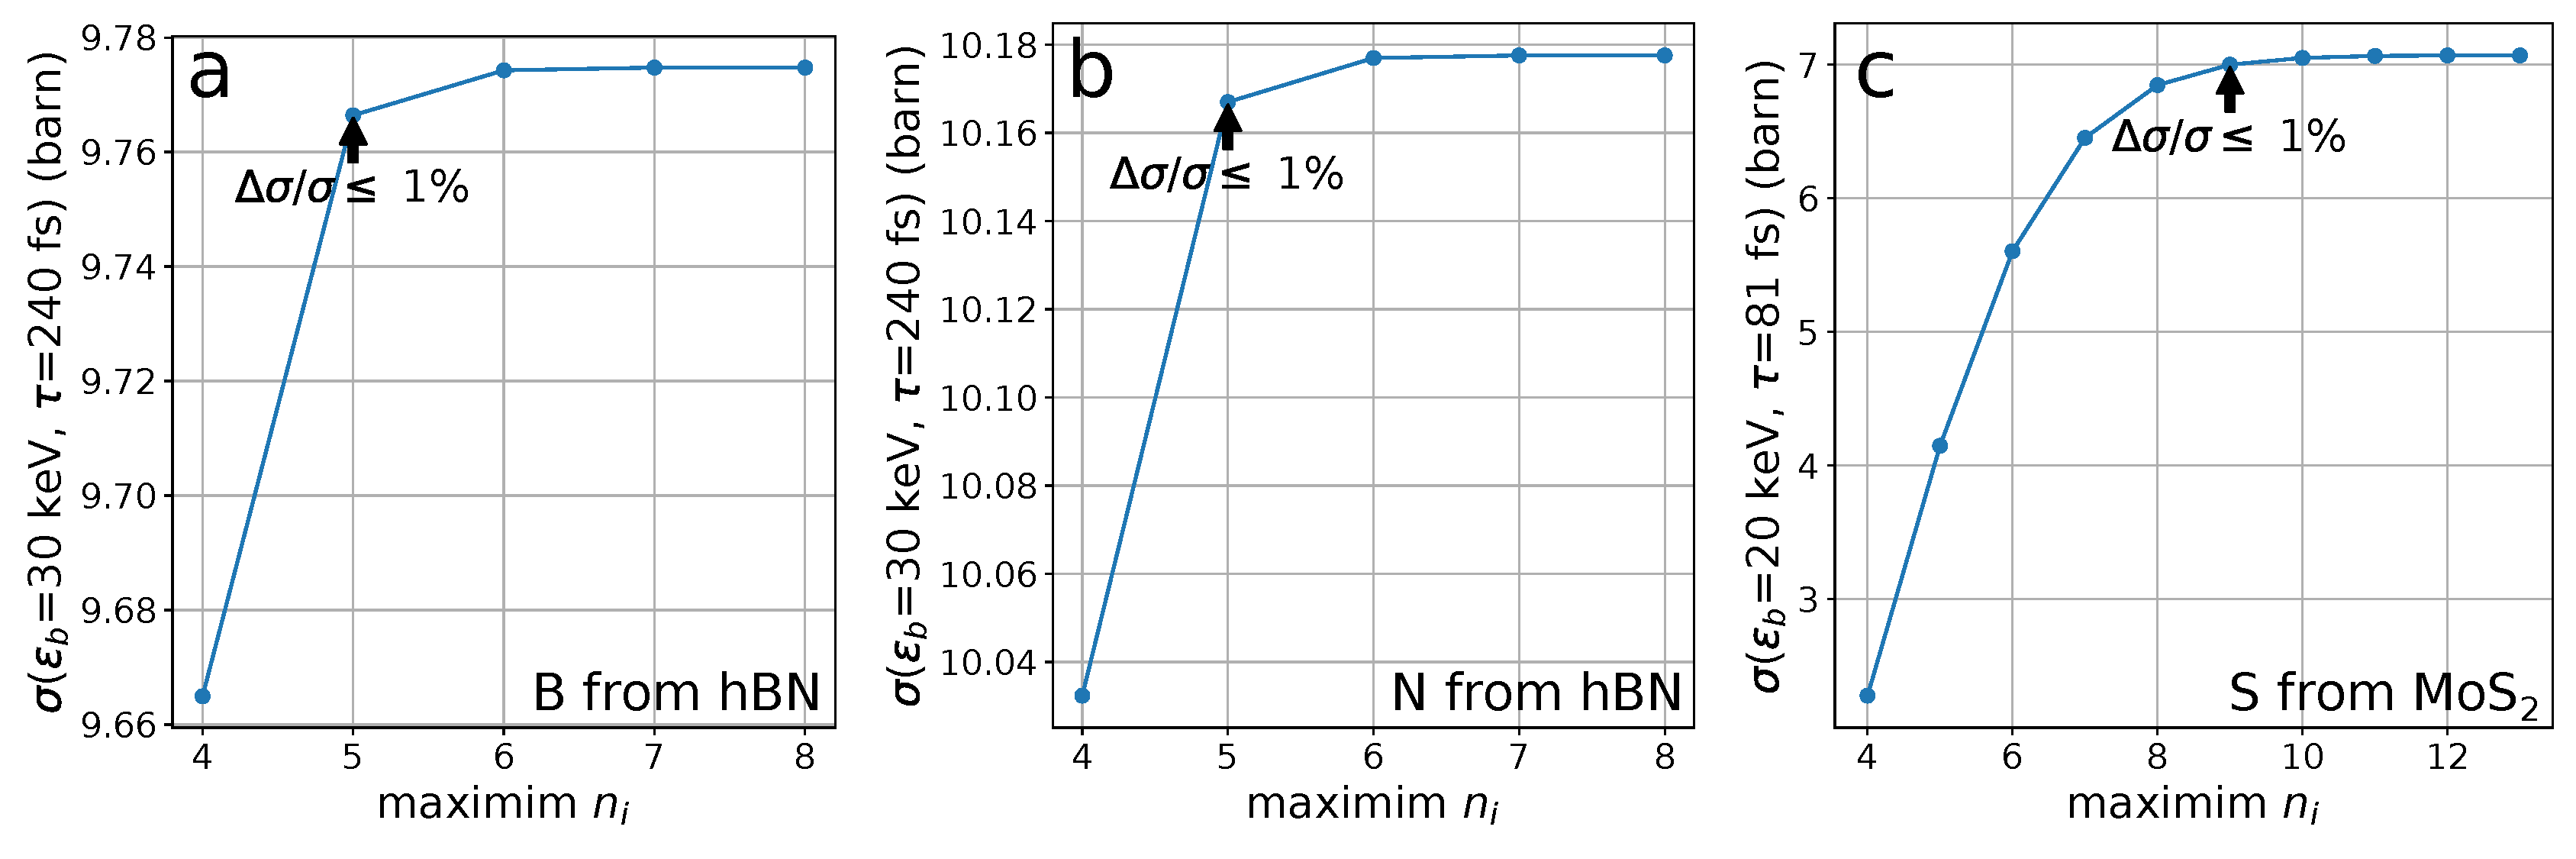
\includegraphics[width=\textwidth]{figures/nimax.pdf}
  \caption{
    Convergence of the sputtering cross section with respect to the maximum
    number of beam-induced excitations $n_i^\text{max}$ considered.
    The simulated beam energies $\epsilon_b$ are the lowest experimental beam
    energies used for each material.
    The excitation lifetimes $\tau$ are those used to fit the experimental data
    in figures \ref{fig:edgeCross} and \ref{fig:MoS2Cross}.
    Each cross section is deemed converged when any increase in $n_i^\text{max}$
    increases the cross section by less than 1\%.
  }
  \label{fig:nimax}
\end{figure}

%------------------------------------------------------------------------------
\pagebreak
\section{Peaks in the sputtering cross section of hBN}
\label{app:edgePeaks}
%------------------------------------------------------------------------------

\begin{figure}[H]
  \centering
  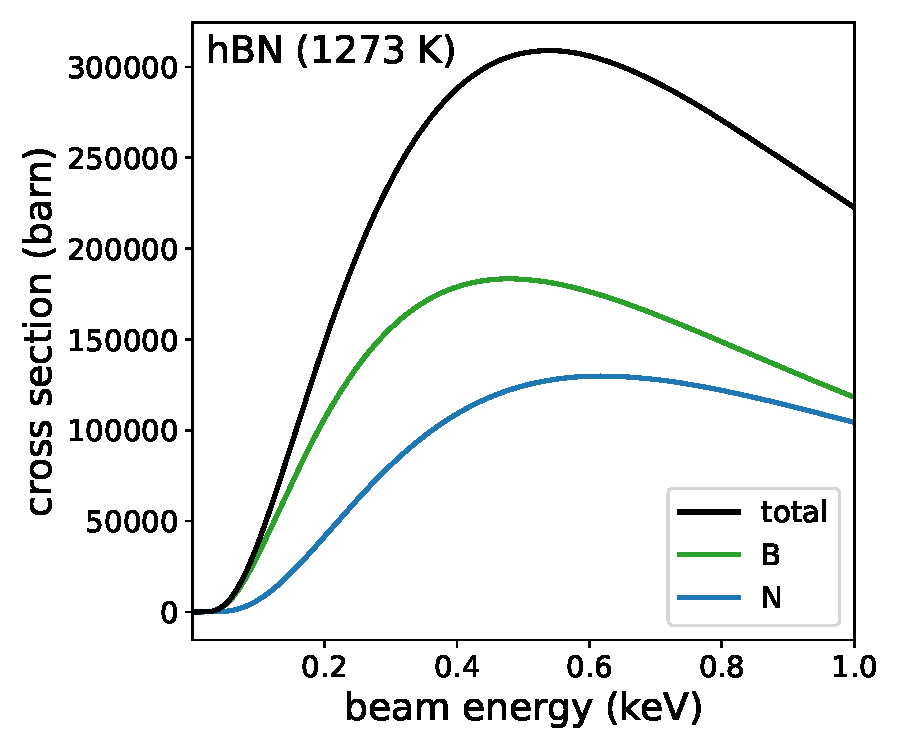
\includegraphics[width=0.6\textwidth]{figures/edgePeaks.pdf}
  \caption{
    The sputtering cross sections of boron and nitrogen from the hBN armchair
    edge peak at beam energies much lower than those typically used for
    microscopy and defect engineering.
    However, as mentioned in the main text, the validity of our perturbative
    approximation to the scattering operator breaks down at low beam energies
    (section \ref{sec:Pi}).
    Thus, the values and positions of these peaks may change if higher order
    perturbation terms are considered.
  }
  \label{fig:edgePeaks}
\end{figure}

%-------------------------------------------------------------------------------
\pagebreak
\section{Fitting and converging $S$}
\label{app:fitting}
%-------------------------------------------------------------------------------

\begin{figure}[H]
  \centering
  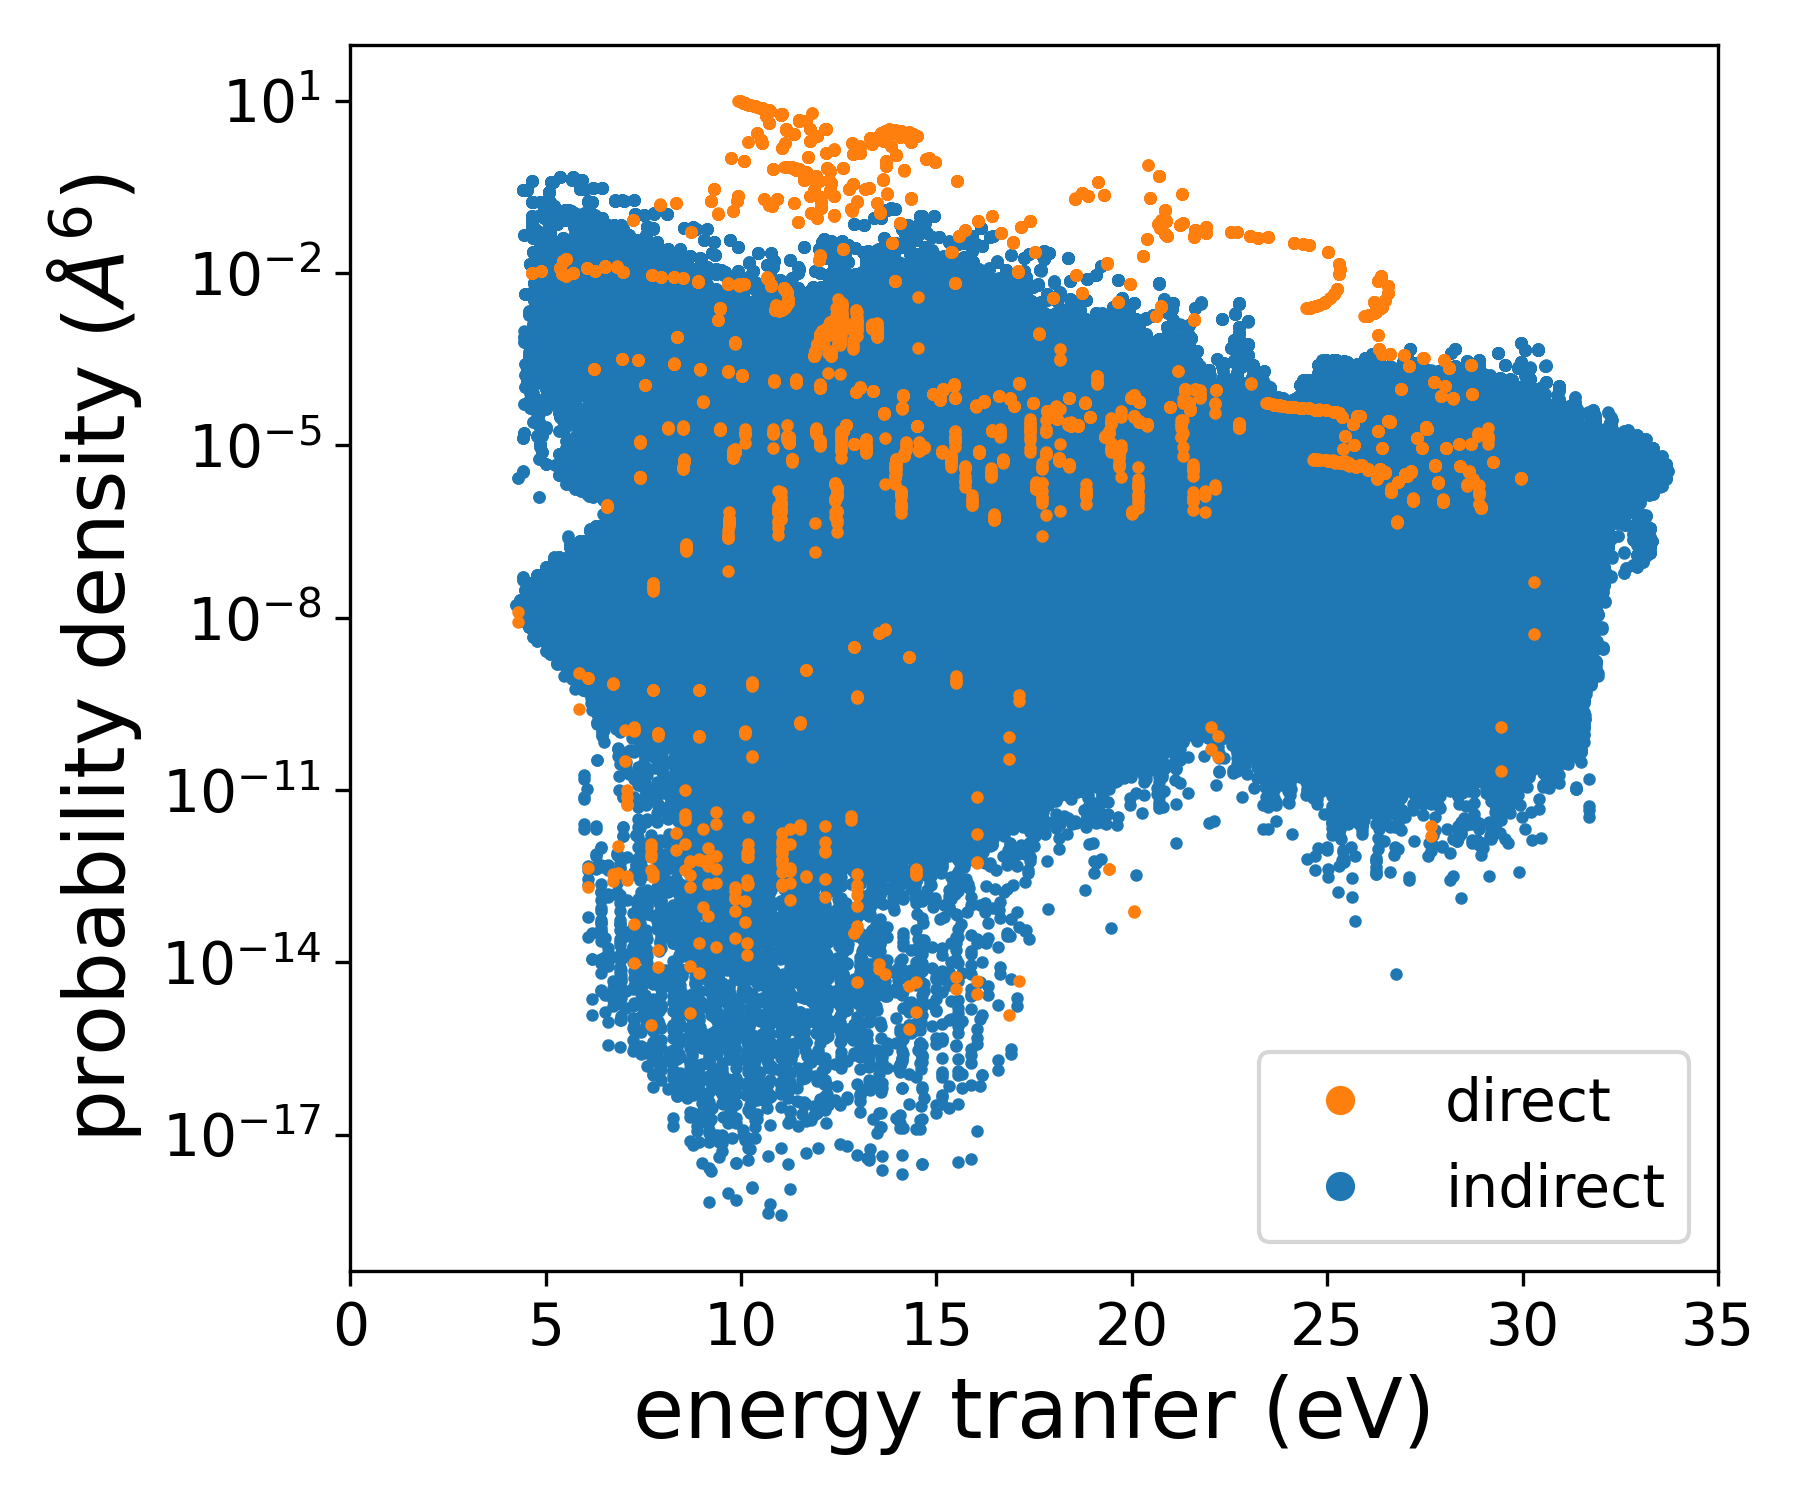
\includegraphics[width=0.6\textwidth]{figures/scatterDirHBN.png}
  \caption{
    The most probable beam-induced electronic excitations are direct
    transitions.
    Each circle denotes the probability density centered on a particular
    excitation instigated by a 40 keV beam electron in hexagonal boron nitride,
    whose Brillouin zone was sampled by a $18\times18\times1$ Monkhorst-Pack
    mesh.
  }
  \label{fig:scatter}
\end{figure}
%
\textcolor{blue}{
As shown in formula (\ref{eq:Pi}), the probability $P_i(\epsilon_b, n_i)$ that
a beam electron of energy $\epsilon_b$ excites a specific number $n_i$ of
material electrons depends solely $S(\epsilon_b)$, the sum of all transition
probabilites defined in equation (\ref{eq:S}).
As such, convergence of $S$ with respect to all simulation parameters is
crucial to calculating the effect of electronic excitation on sputtering.
In this section, we describe the general scheme that we use to converge $S$
with respect to our simulation parameters.
In particular, the convergence with respect to k-point density must be treated
with care, and will be the primary focus of the remainder of this section.
}

Because the square of the momentum transfer appears in the denominator of the
$t$-channel in equation (\ref{eq:M}), the probability density for electronic
excitation peaks sharply when the momentum transfer is minimized.
This minimization occurs when the beam electron induces a direct transition,
in which the resulting electron and hole lie on the same k-point.
Thus, direct excitations that conserve crystal momentum tend to be much more
likely than indirect excitations (figure \ref{fig:scatter}).

As a result, a sparse k-point mesh leads to an overestimation of $S$.
% the sum of all transition probabilities defined in equation (\ref{eq:S}).
This is because a coarser k-point mesh yields a higher proportion of direct
transitions, as there are fewer indirect transitions available for each
k-point.
For a given number of k-points $N_k$, the number direct transitions is
proportional to $N_k$, while the number of indirect transitions is proportional
to $N_k^2$.
Thus, increasing $N_k$ increases the proportion of possible indirect
transitions, lowering $S$.
For a sufficiently dense mesh, the distinction between direct and nearly direct
transitions is inconsequential, in which case, $S$ is converged with respect to
$N_k$.

\begin{figure}[H]
  \centering
  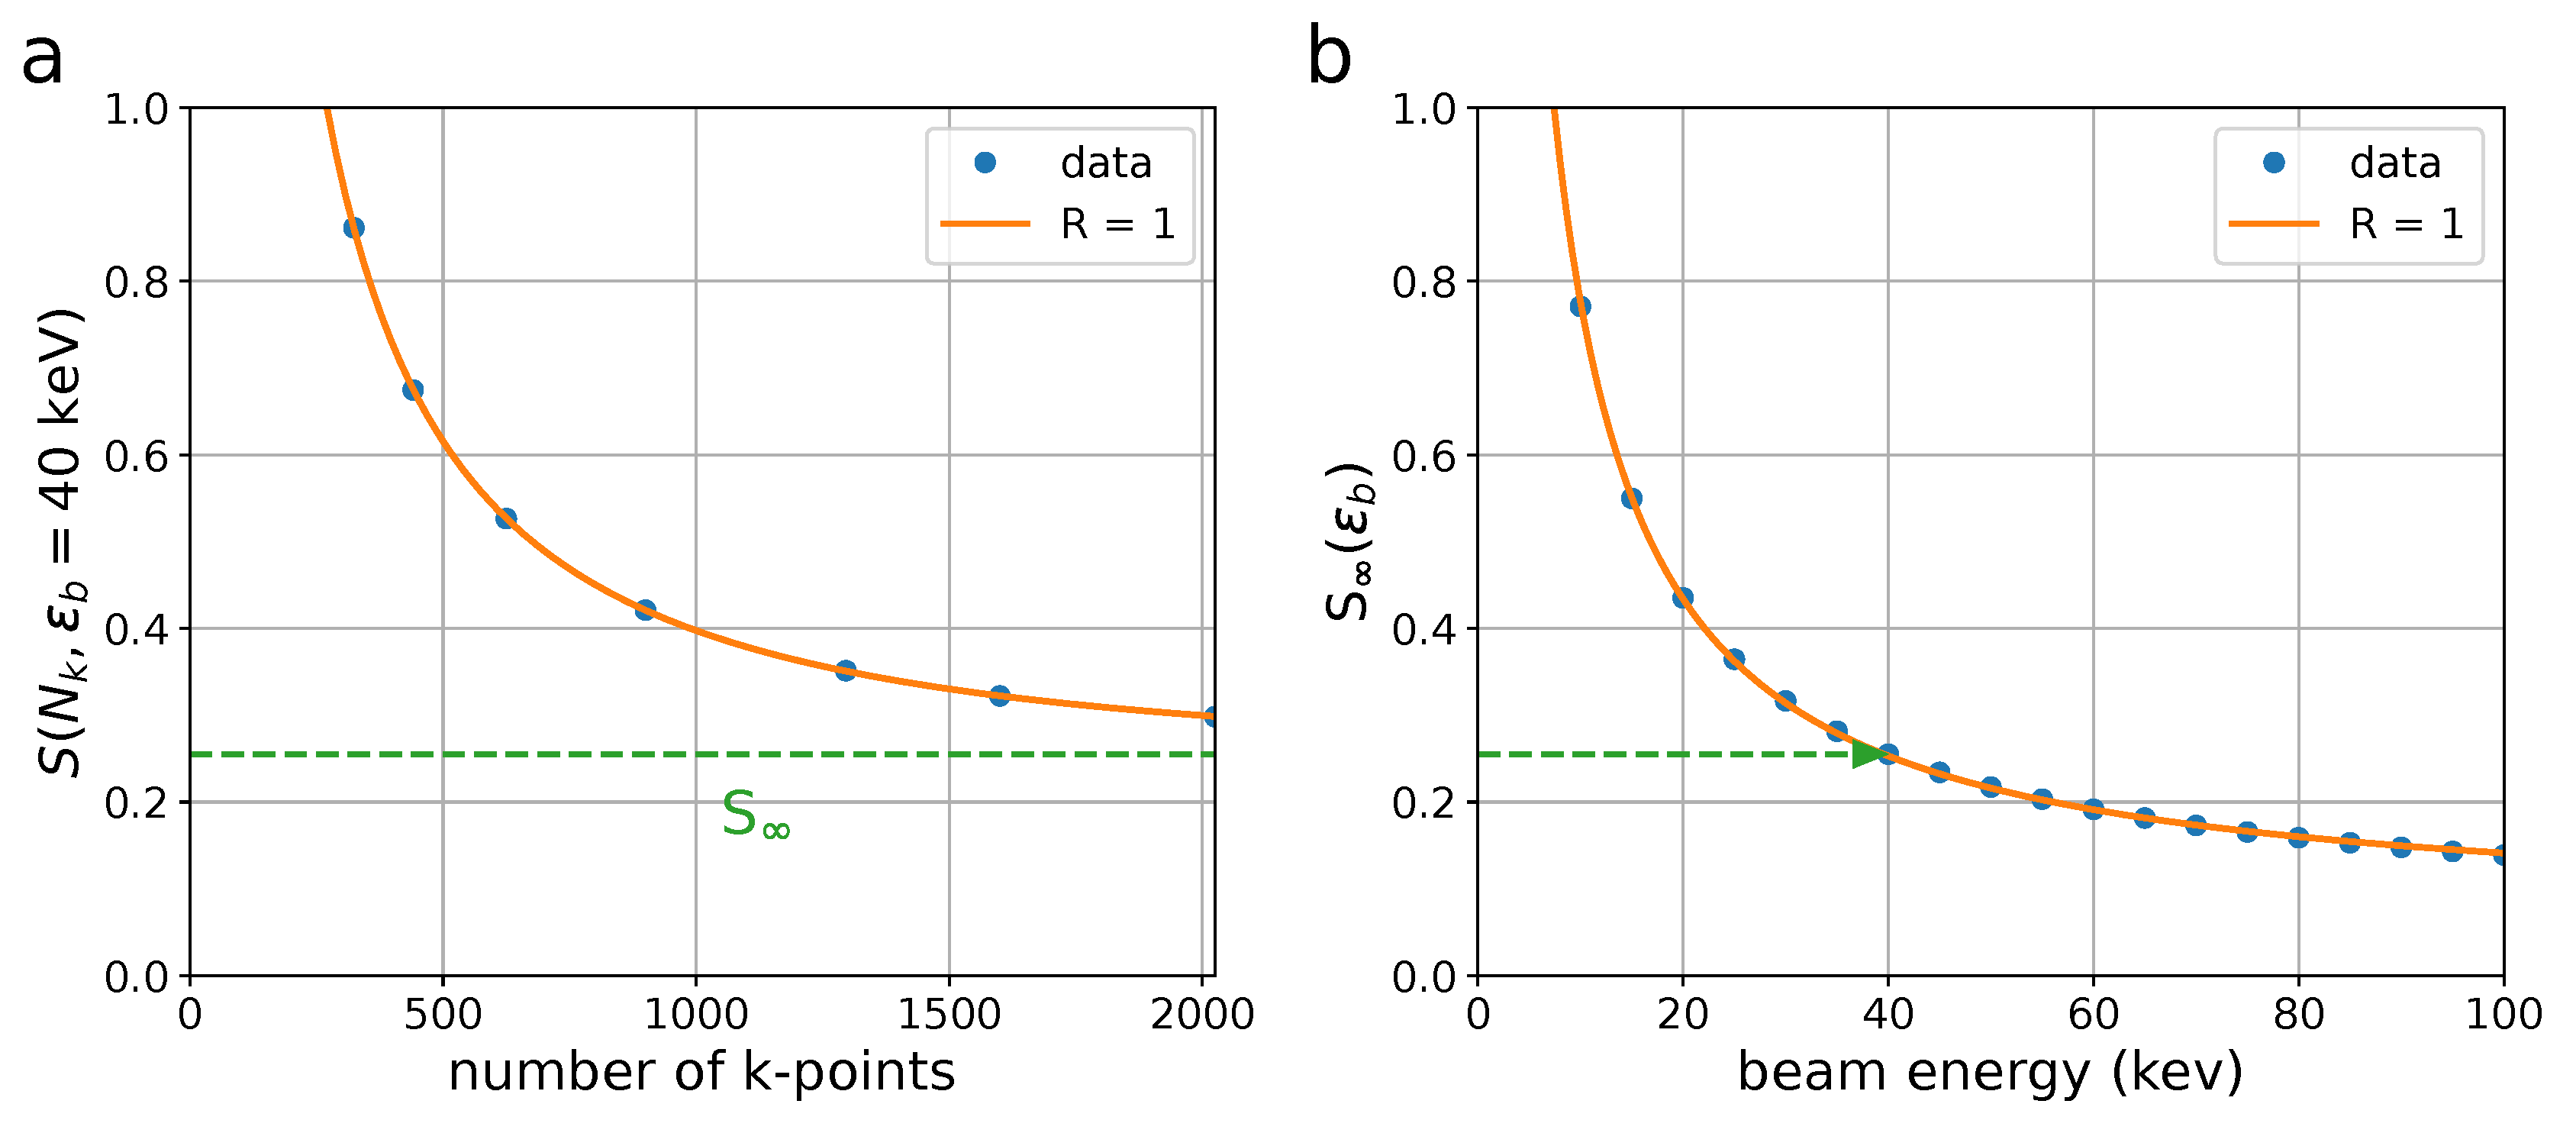
\includegraphics[width=\textwidth]{figures/sum.pdf}
  \caption{
    Finding the large crystal limit of $S(\epsilon_b)$ requires extrapolation.
    Panel (a) shows the dependence of $S$ on the number k-points $N_k$ in the
    Brillouin zone of hBN under 40 keV irradiation.
    The simulated points are fitted well by equation (\ref{eq:SNk}).
    The green dashed line denotes $S_\infty$, the asymptotic limit of $S(N_k)$
    for large $N_k$.
    Panel (b) then shows the dependence of $S_\infty$ on the beam energy
    $\epsilon_b$, which is fitted well by equation (\ref{eq:SEb}).
    The green arrow in panel (b) illustrates how $S_\infty(\epsilon_b=40\text{
    keV})$ is determined by the fit in panel (a).
    \textcolor{blue}{
    The fitted curve in panel (b) is then used as $S(\epsilon_b)$ in formula
    (\ref{eq:Pi}) to calculate $P_i$ for hBN.
    The same fitting and extrapolation method is used for MoS$_2$.
    }
  }
  \label{fig:Sfit}
\end{figure}

Satisfactory convergence of $S$ requires an extremely dense k-point mesh.
We therefore use extrapolation to determine the converged value of $S$.
For a given beam energy $\epsilon_b$, we calculate $S$ for various $N_k$.
We then fit the points to a curve of the form

\begin{equation}
  S(N_k, \epsilon_b)
  =
  \frac{a}{N_k-b}e^{-cN_k} + S_\infty,
  \label{eq:SNk}
\end{equation}
%
where $a$, $b$, $c$, and $S_\infty$ are all fitting parameters that depend on
$\epsilon_b$ (figure \ref{fig:Sfit}a).
The last parameter $S_\infty$ is the limit of $S$ for large $N_k$, and is taken
as the converged value of $S$ for that beam energy.
We repeat this for multiple values of $\epsilon_b$ ranging from 5 to 100 keV
and record the best fit
$S_\infty$ for each
% and then use equation (\ref{eq:SNk}) to determine
$\epsilon_b$.
Based on the work of Bethe,\cite{Bethe1930, Susi2019, Kretschmer2020} we fit
the resulting values of $S_\infty(\epsilon_b)$ to an inverse function,

\begin{equation}
  S_\infty(\epsilon_b)
  =
  \frac{A}{\epsilon_b - B} + C.
  \label{eq:SEb}
\end{equation}
%
where $A$, $B$, and $C$ are fitting parameters.
The parameters for hBN and MoS$_2$ are given in table \ref{tab:fit}.
The fitted curve can then be substituted for $S(\epsilon_b)$ in formula
(\ref{eq:Pi}) to obtain $P_i(\epsilon_b, n_i)$.
% the probability of exciting $n_i$ electrons in the large crystal limit.

\begin{table} \centering 
  \begin{tabular}{lccc}
    \toprule
    material &A (keV) &B (keV) &C \\
    \midrule
    hBN     &7.655 &-0.770 &0.06526 \\
    MoS$_2$ &49.05 &-3.867 &0.3547 \\
    \bottomrule
  \end{tabular}
  \caption{
    Fitting parameters of equation (\ref{eq:SEb}) for hBN and MoS$_2$.
  } 
\label{tab:fit}
\end{table}

% Finally, $S$ is also converged with respect to all other parameters.
% These include the maximum virtual photon momentum, DFT cutoff energy, and
Finally, $S$ is also converged with respect to the maximum virtual photon
momentum, DFT cutoff energy, and height of the pristine unit cell (figure
\ref{fig:convergences}).
In these cases, $S$ is considered converged with respect to a parameter
when any increase in the parameter's precision changes $S$ by less than 5\%.
% \textcolor{blue}{
% We found that the converged value of a given parameter was insensitive to the
% k-point density.
% For example, a cutoff energy of 299 eV in hBN converged $S$ for both
% $6\times6\times1$ and $12\times12\times1$ meshes.
% We therefore performed all of these convergence calculations using a
% $6\times6\times1$ k-point mesh.
% }

\begin{figure}[H]
  \centering
  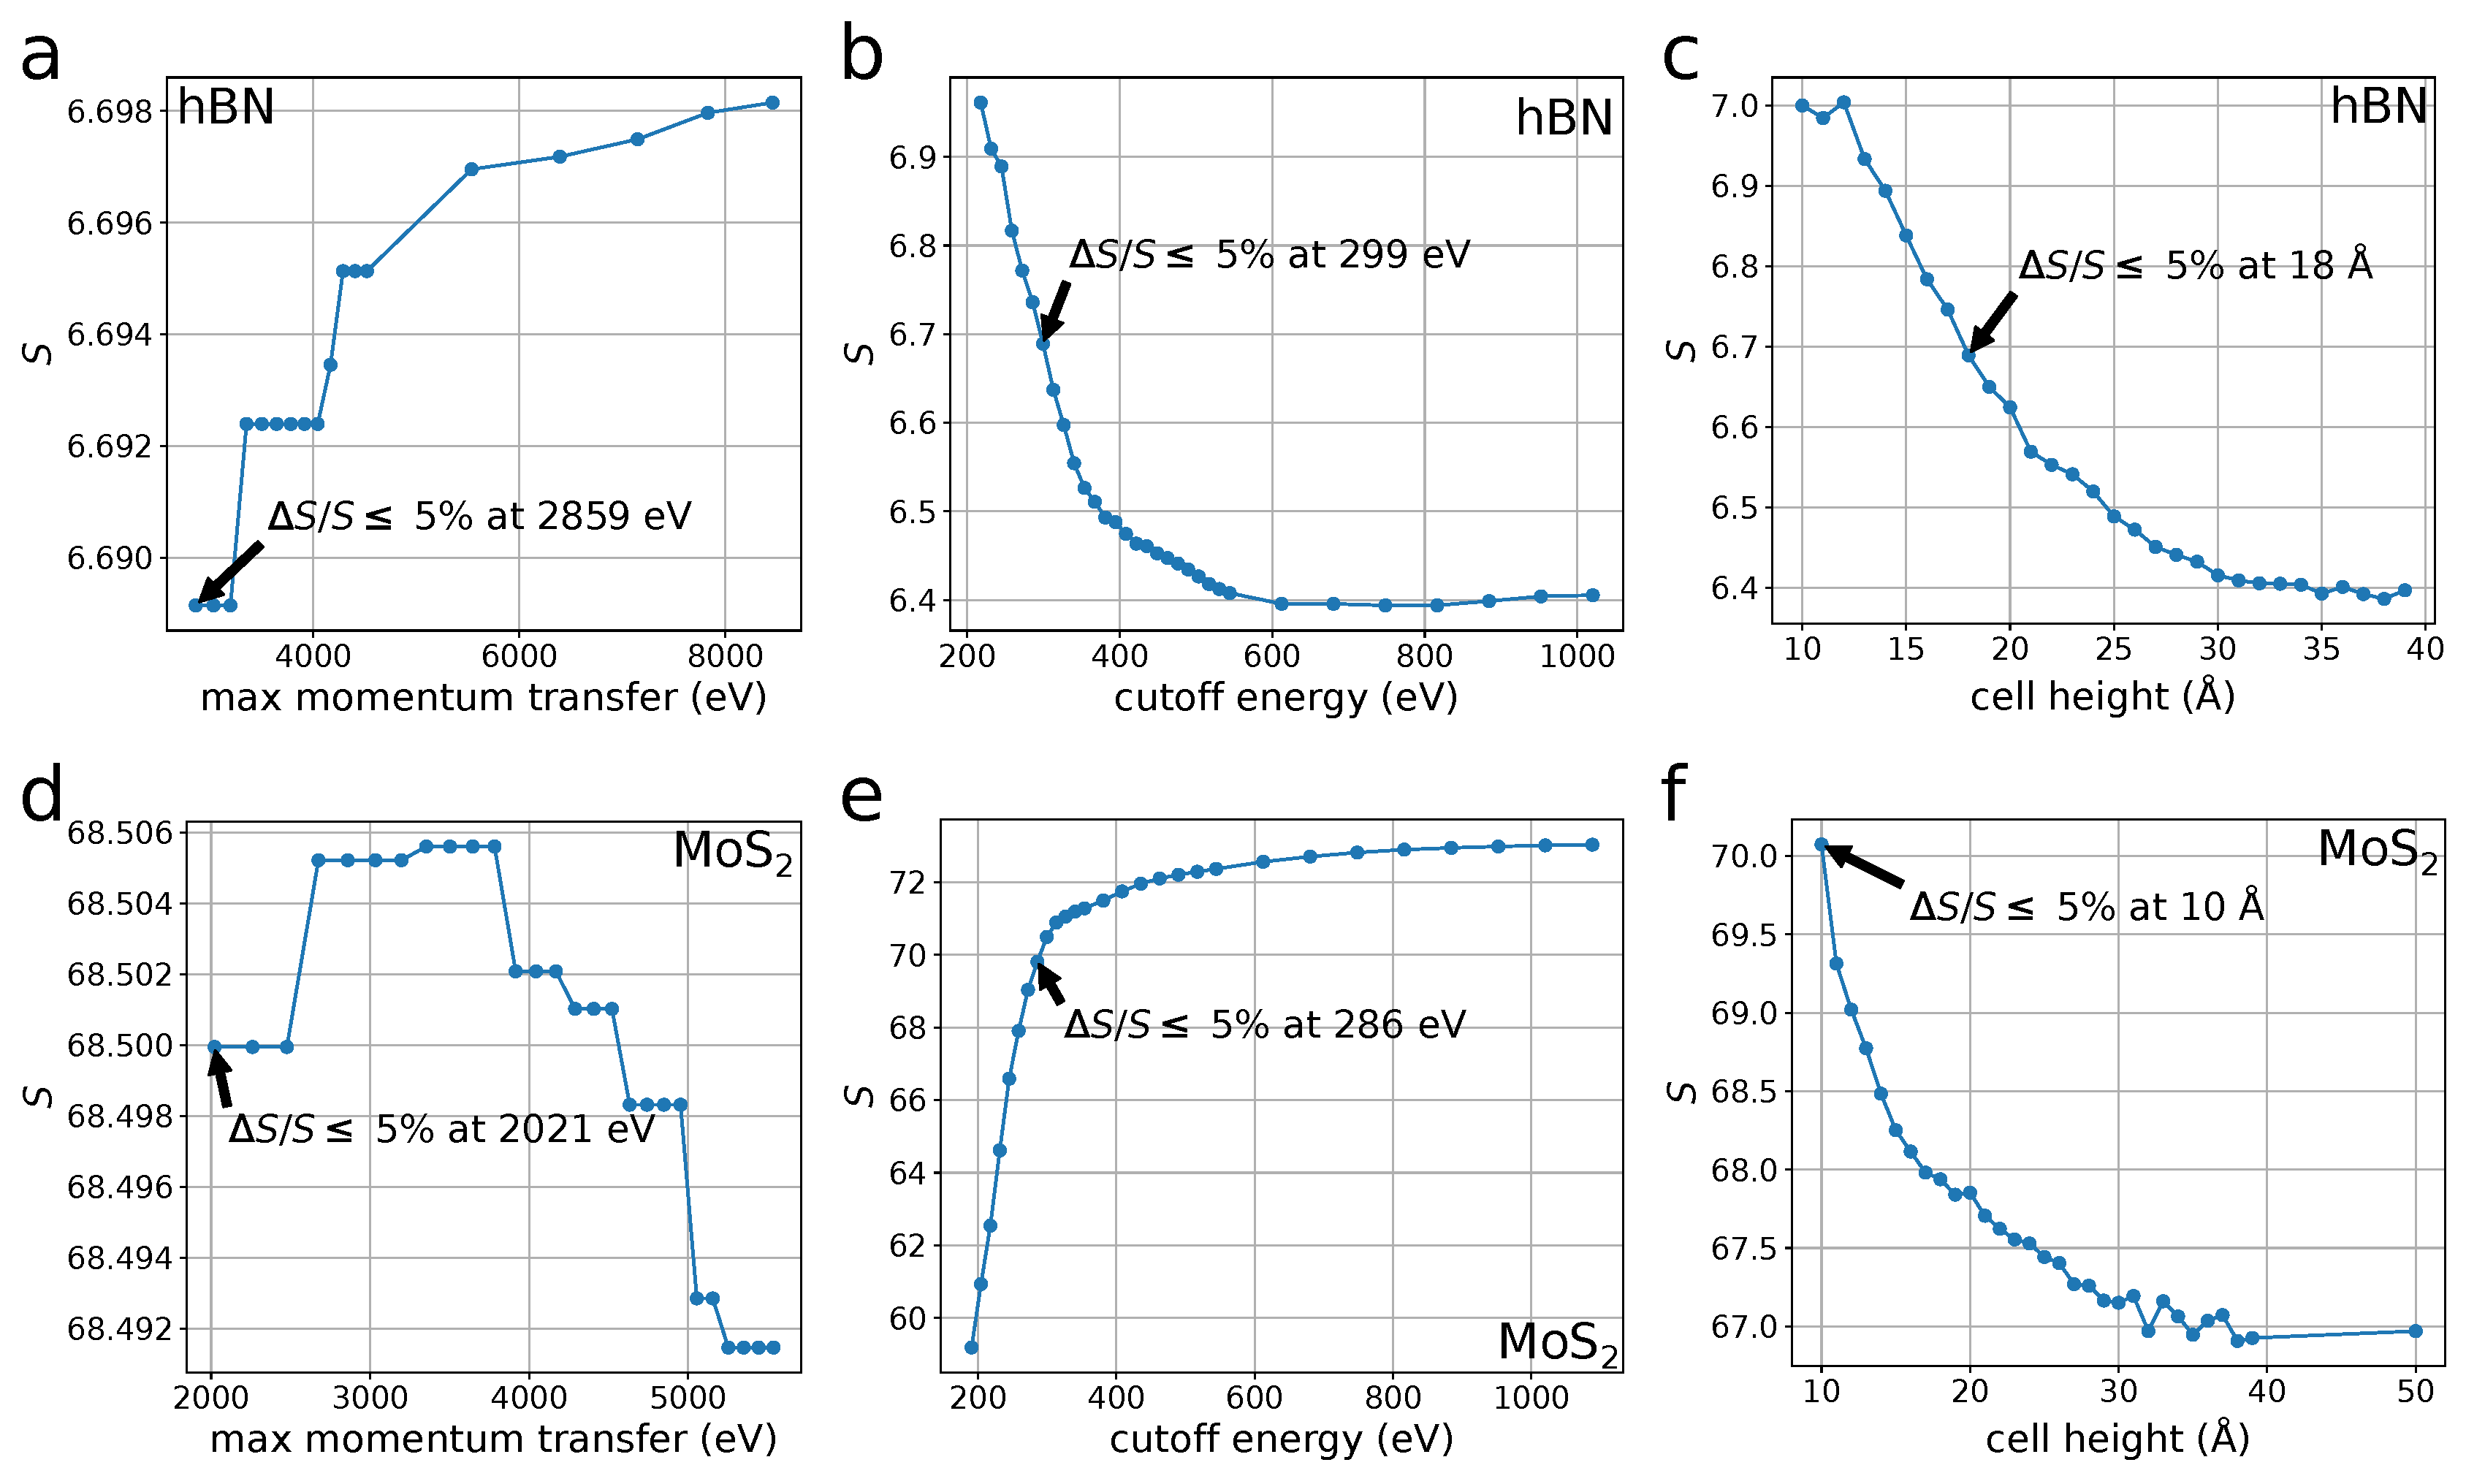
\includegraphics[width=\textwidth]{figures/convergences.pdf}
  \caption{
    Convergence of $S$ with respect to the (a and d) maximum magnitude of
    virtual photon momentum considered, (b and e) plane-wave DFT cutoff energy,
    and (c and f) height of the unit cell.
    A $6\times6\times1$ k-point mesh and a beam energy of 60 keV is used to
    generate all six plots.
    The converged parameters were found to be insensitive to changes in k-point
    density and beam energy.
    $S$ is deemed converged when any increase in precision changes $S$ by less
    than 5\%.
  }
  \label{fig:convergences}
\end{figure}
\break

%------------------------------------------------------------------------------
\pagebreak
\section{Validity of the three simplifying assumptions}
\label{app:assumptions}
%------------------------------------------------------------------------------

While the three assumptions laid out in section \ref{sec:assumptions} may seem
drastic, their affect on the sputtering cross section is small due to a
cancellation of errors.
To see this, consider the connection between the potential energy
surfaces (ESs) and the PKA velocity.
% This connection underpins all three simplifying assumptions.
By assumption 1, the ESs at the PKA’s initial position are equally spaced,
separated by the material's band gap.
By assumption 2, the ESs converge to the same energy as the PKA
approaches a distance $d$.
We shall ignore assumption 3 for now.
If we consider that the ESs are not constant as the PKA moves towards $d$, so
that the PKA slows down in transit, then the energy required to get to $d$
depends on when the system relaxes to a lower ES.
This is because higher ESs have shallower slopes than do the lower ones, so
the PKA's deceleration will be smaller while on a higher ES.
Thus, as the PKA moves, the ESs converge by assumption 2, and the energy lost
during relaxation tends to shrink.

% This is where the error cancellation occurs.
By introducing assumption 3, the energy lost during relaxation does not
shrink but remains constant while the PKA sputters, and is therefore generally
greater than it would be with gradually changing ESs.
% This disparity grows the longer the system remains excited.
Our method therefore overestimates the energy lost during relaxation.
On the other hand, because the PKA does not slow down until it reaches $d$,
assumption 3 also underestimates the sputtering time $t_s$, introduced in
equation (\ref{eq:R}).
A smaller $t_s$ means that fewer excitations relax during sputtering,
increasing the cross section.
However, each relaxation comes at a higher energy cost, which makes the PKA
less likely to overcome the displacement threshold, decreasing the cross
section.
Thus, the underestimation $t_s$ counteracts the overestimation of the energy
lost during relaxation, so that final effect on the sputtering cross section is
small.

Considering the ESs also sheds light on the computational cost saved by
assumption 3.
Without assumption 3, $t_s$ would depend on the exact times that each
relaxation occurs.
In this case, calculating the cross section would require integration over time
for each excited ES considered.
We have found that the consideration of 5 and 9 excited ESs are necessary to
converge the cross sections of hBN and MoS$_2$ respectively (figure
\ref{fig:nimax}).
For an N-point Gaussian quadrature, this would multiply the computational costs
by $N^5$ and $N^9$ respectively.
Assumption 3 removes this complication by eliminating the need to consider
exactly when each relaxation happens.
Instead, only the total number of relaxations before the PKA reaches $d$ need
be considered.
% By employing assumption 3, only consider the total number of relaxations before
% the PKA reaches $d$ need be considered, regardless of when those relaxations
% occur.

%------------------------------------------------------------------------------
\pagebreak
\section{Calculating $E_\text{min}$}
\label{app:Emin}
%------------------------------------------------------------------------------

\begin{figure}[H]
  \centering
  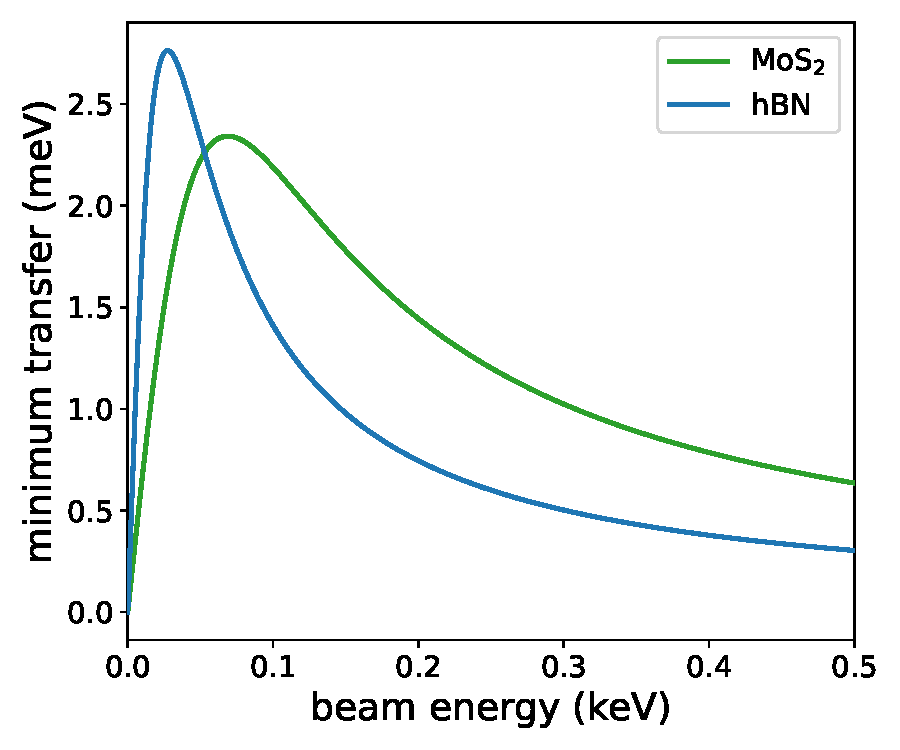
\includegraphics[width=0.6\textwidth]{figures/emin.pdf}
  \caption{
    The minimum energy transfer from the beam electron to the target nucleus
    peaks at very low beam energies and is always much smaller than the
    nuclei's average thermal kinetic energy of $\sim$39 meV at room
    temperature. 
  }
  \label{fig:Emin}
\end{figure}

In hBN, a unit cell contains a boron and nitrogen atom.
As these atoms have similar masses and displacement thresholds (table
\ref{tab:Ed}), the sputtering of both atoms should be considered for a given
beam energy.
Thus, we approximate the maximum cross sectional area $\sigma_\text{max}$ of
these atoms to be $\Omega_\text{hBN}/2$, where $\Omega_\text{hBN}$ is the area
of the hBN unit cell.
On the other hand, molybdenum is much heavier than sulfur and has a much larger
displacement threshold in MoS$_2$.\cite{Komsa2012}  
This means that only the sputtering of sulfur needs to be considered.
Additionally, of the two sulfur atoms in the MoS$_2$ unit cell, only the atom
on the outgoing surface is eligible to sputter from a pristine system.
\cite{Komsa2012}
Therefore, $\sigma_\text{max}$ for sulfur sputtering from MoS$_2$ is
$\Omega_\text{MoS$_2$}$, the area of the MoS$_2$ unit cell.

To approximate $E_\text{min}$, we use the Rutherford displacement cross section
\cite{Thornton2004, Sakurai2011, Yoshimura2018} as an approximation to equation
(\ref{eq:basicSigma}),

\begin{equation}
  \sigma_R
  =
  \pi\left(\frac{Z\alpha}{|\mathbf{p}|\beta}\right)^2
  \left(\frac{E_\text{max}}{E_d} - 1\right).
  \label{eq:Rutherford}
\end{equation}
%
Setting $\sigma_R=\sigma_\text{max}$ and $E_d=E_\text{min}$ and solving for
$E_\text{min}$ yields

\begin{equation}
  E_\text{min}(\epsilon_b)
  =
  E_\text{max}
  \left[\frac{\Omega}{\pi}
    \left(\frac{|\mathbf{p}_b|\beta}{Z\alpha}\right)^2 + 1
  \right]^{-1}.
  \label{eq:Emin}
\end{equation}
%
Using the Rutherford cross section instead of the McKinley-Feshbach cross
section should be accurate for small beam energies for which $\beta\ll 1$.
This makes it well-suited for finding $E_\text{min}$, since
$E_d(n_f)<E_\text{min}$ only for large $n_f$, and large $n_i$ (and thus $n_f$)
are much more likely for small beam energies (figure \ref{fig:Pi}).

With that said, the sputtering cross section is fairly insensitive to the exact
value of $E_\text{min}$ when $E_\text{min} \ll E_\text{max}$.
This is because the post-collision velocity of the PKA diminishes when the
energy transfer $E$ shrinks.
The beam-induced excitations therefore have more time to relax before the PKA
reaches the step in the energy surface (section \ref{sec:assumptions}).
This makes $P_f$ small for small $E$, so that contributions to the integral in
equation (\ref{eq:totSigma}) are extremely tiny for $E$ near $E_\text{min}$.
As a result, changes in $E_\text{min}$ are essentially immeasurable for beam
energies greater than 1 keV.
Nonetheless, the use of $E_\text{min}$ is necessary for the calculation of a
finite sputtering cross section.

\bibliography{library}
\bibliographystyle{rsc}

\end{document}
